\section{Wordpress}
\label{sec:CMS_wp}

WordPress is a free and open-source content management system (CMS) based on PHP and MySQL. \cite{cms_wp_over} Features include a plugin architecture and a template system. WordPress was used by more than 23.3\%of the top 10 million websites as of January 2015. WordPress is the most popular blogging system in use on the Web, at more than 60 million websites \cite{cms_wp_stats}.


\subsection{History}
\label{subsec:wp_his}
It was first released on May 27, 2003, by its founders, Matt Mullenweg and Mike Little, as a fork of b2/cafelog. The license under which WordPress software is released is the GPLv2 (or later) from the Free Software Foundation.
b2/cafelog, more commonly known as simply b2 or cafelog, was the precursor to WordPress. b2/cafelog was estimated to have been installed on approximately 2,000 blogs as of May 2003. It was written in PHP for use with MySQL by Michel Valdrighi, who is now a contributing developer to WordPress. Although WordPress is the official successor, another project, b2evolution, is also in active development.
WordPress first appeared in 2003 as a joint effort between Matt Mullenweg and Mike Little to create a fork of b2. Christine Selleck Tremoulet, a friend of Mullenweg, suggested the name WordPress.
In 2004 the licensing terms for the competing Movable Type package were changed by Six Apart, resulting in many of its most influential users migrating to WordPress. By October 2009 the Open Source CMS MarketShare Report concluded that WordPress enjoyed the greatest brand strength of any open-source content-management system \cite{cms_wp}. 



\subsection{Themes}
\label{subsec:wp_themes}


WordPress has a web template system using a template processor.
WordPress users may install and switch between themes. Themes allow users to change the look and functionality of a WordPress website and they can be installed without altering the content or health of the site. Every WordPress website requires at least one theme to be present and every theme should be designed using WordPress standards with structured PHP, valid HTML and CSS. Themes may be directly installed using the WordPress Appearance administration tool in the dashboard or theme folders may be uploaded via FTP. The PHP, HTML (HyperText Markup Language) and CSS (Cascading Style Sheets) code found in themes can be added to or edited for providing advanced features. WordPress themes are in general classified into two categories, free themes and premium themes. All the free themes are listed in the WordPress theme directory and premium themes should be purchased from marketplaces and individual WordPress developers. WordPress users may also create and develop their own custom themes if they have the knowledge and skill to do so. If WordPress users do not have themes development knowledge then they may download and use free WordPress themes from wordpress.org \cite{cms_wp}. 

\subsection{Plugins}
\label{subsec:wp_plugins}


WordPress's plugin architecture allows users to extend the features and functionality of a website or blog. WordPress has over 39,078 plugins available, each of which offers custom functions and features enabling users to tailor their sites to their specific needs. These customizations range from search engine optimization, to client portals used to display private information to logged in users, to content displaying features, such as the addition of widgets and navigation bars. But not all available plugins are always abreast with the upgrades and as a result they may not function properly or may not function at all \cite{cms_wp}.



\begin {figure}[h]
\graphicspath{{images/chapter_cms/}}
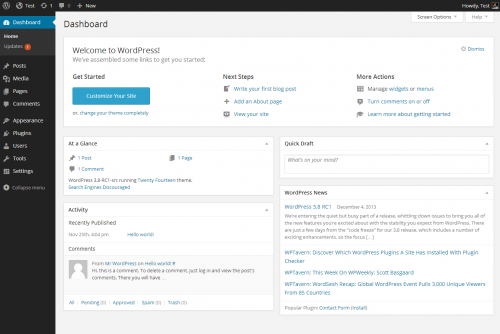
\includegraphics[width=\textwidth]{wp_dash}
\caption{WordPress Dashboard}
\end {figure}
